\chapter{Astronomy Big Data}


Big data are high-volume, high-velocity, and/or high-variety information assets that require new forms of processing to enable enhanced decision making, insight discovery and process optimization. Examples of big data include information such as Web search results, electronic messages (e.g. SMS, email and instant messages), social media postings, pictures, videos and even system log data. However, it can also include cash transactions, check images, receipts and other transactional information depending on the source of the information. \\

Astronomical datasets are growing at an exponential rate: high performance computing applications in astronomy are enabling complex simulations with many billions of particles, while the forthcoming generation of telescopes will collect data at rates in excess of terabytes per day. This data deluge, both now and into the future, presents some critical challenges for the way astronomers derive new knowledge from their data.\\

In this chapter, we make an overview of some of the greatest telescopes, the way they acquire and store data and the problem they face.


\section{Atacama Large Millimiter Array}

\subsection{ALMA Instrument}

ALMA is a worldwide project; the synthesis of early visions of astronomers in its three partner communities: Europe, North America and Japan.\\

ALMA is a fusion of ideas, with its roots in three astronomical projects: the Millimeter Array (MMA) of the United States, the Large Southern Array (LSA) of Europe, and the Large Millimeter Array (LMA) of Japan.\\

\begin{figure}[H]
\centering
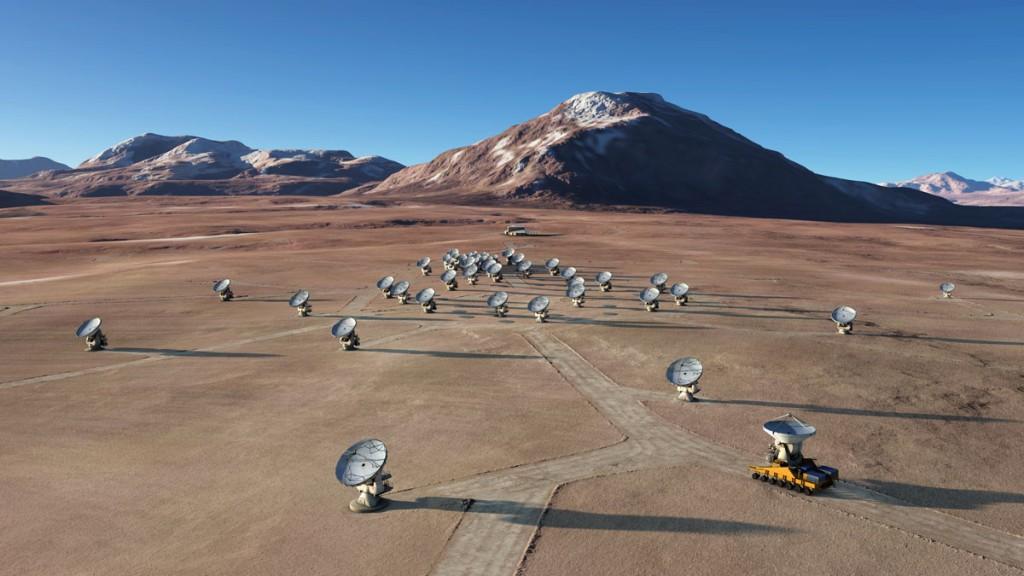
\includegraphics[width=11cm,height=8cm]{images/alma.jpg}\\
\caption{ALMA dishes in Atacama Desert}
\end{figure}


\textbf{Millimeter Array} \\

The origins of the Millimeter Array (MMA) are found in the science of the NRAO 36-Foot Telescope (later known as the 12-Meter Telescope), soon followed by the 4.9m telescopes at the University of Texas and Aerospace Corporation, the 14m telescope at the Five Colleges Radio Astronomical Observatory, and the 7m telescope at AT\&T Bell Labs. The science targets of the MMA included the same broad range of topics seen at the VLA: (NSF) in July, 1990, called for an array of 40 antennas of 8-meter diameter, with four receiver bands covering the atmospheric windows from 30-350 GHz, configurable in four arrays of size 70-3000 m. The proposal discussed two possible sites for the MMA, both in the southwestern United States. Studies of the atmospheric transparency and phase stability at these sites led to similar studies on Mauna Kea, in Hawaii.\\

Concerns with the limited size of the area available to the MMA on Mauna Kea and with potential environmental problems prompted a search for potential sites in Chile. From April 1994, many highelevation sites were visited. Finally, the site retained for the MMA was formally proposed in 1996: it was the Chajnantor plateau. \\

This effort culminated in the signing of the ALMA Agreement on February 25, 2003, between the North American and European parties. More than 14 government agencies in Chile were involved in the negotiations.\\

Assuming all three partners are able to meet their commitments, it was decided that the final project would be cost-shared 37.5\% / 37.5\% / 25\% between North America, Europe, and Japan, respectively. The observing time, after a 10\% share for Chile, would be shared accordingly.\\

ALMA is an instrument that consist of a giant array of 12-m antennas with baselines up to 16 km, and an additional compact array of 7-m and 12-m antennas to greatly enhance ALMA's ability to image extended targets, located on the Chajnantor plateau at 5000m altitude. Initially, it will observe at wavelengths in the range $3 mm$ to $400 μm$ ($84$ to $720 GHz$). The antennas can be moved around, in order to form arrays with different distributions of baseline lengths. More extended arrays will give high spatial resolution, more compact arrays give better sensitivity for extended sources. In addition to the array of 12-m antennas, there is the Atacama Compact Array (ACA), consisting of twelve 7-m antennas and four 12-m antennas. This array will mostly stay in a fixed configuration and is used to image large scale structures that are not well sampled by the ALMA 12-m array.\\

The design of ALMA is driven by three key science goals:

\begin{itemize}

\item The ability to detect spectral line emission from CO in a normal galaxy like the Milky Way at a redshift of $z=3$, in less than 24 hours

\item The ability to image the gas kinematics in protostars and in protoplanetary disks around young Sun-like stars in the nearest molecular clouds ($150 pc$)

\item The ability to provide precise high dynamic range images at an angular resolution of $0.1 arcsec$
\end{itemize}
 
ALMA delivers data cubes, of which the third axis is frequency. In this sense, the final data products are very much like that of an integral field unit with up to a million Spectral Pixels.\\

\textbf{Interferometry}\\
In order to obtain images, the raw visibility data need to be Fourier transformed. When ALMA is in full operations, this imaging step, as well as various calibration steps, will be done in the data reduction pipeline. Thus, fully calibrated data cubes will be delivered to the user.\\

\textbf{Observing frequencies}\\
The frequency range available to ALMA is divided into different receiver bands. Data can only be taken in one band at a time. These bands range from band 3, starting at$ 84 GHz$, to band 10, ending at $\sim950 GHz$.\\

\textbf{Field of view}\\
The FWHM of the ALMA primary beam is 21" at $300 GHz$, and scales linearly with wavelength (diffraction limit of a single 12-m antenna, as opposed to that of the whole array).\\

\textbf{Spatial resolution}\\
The spatial resolution of ALMA depends on the observing frequency and the maximum baseline of the array, following the $1.2 x \Lambda/D$ scaling. In the most compact configurations ($\sim150 m$), resolutions range from 0.7" at $675 GHz$ to 4.8" at $110 GHz$.\\

\textbf{Array configurations}\\
The ALMA 12-m array will cycle from its most compact configuration, with maximum baselines of $\sim~150 m$, to its most extended configuration, with maximum baselines of $\sim 16 km$ (when completed), and back.\\

\textbf{Spectral resolution}\\
ALMA can deliver data cubes with up to 7680 frequency channels (spectral resolution elements). The width of these channels can range between $3.8 kHz$ and $15.6 MHz$, but the total bandwidth cannot exceed $8 GHz$.\\

\subsection{ALMA Science Archive}

As stated in \cite{Etoka12}, the purpose of the ALMA archive is to provide services for:

\begin{itemize}
\item Persistent archiving and retrieval for observacional data.
\item Observaction descrpitors.
\item Datacubes produced by pipeline.
\item Technical and environmental data.
\end{itemize}

And the key-point of the conceptual design of the ALMA Archive is to guarantee that three ALMA Regional Centres (ARCs) hold an identical copy of the archive at the Joint ALMA Observatory (JAO) in Santiago. \\

Relational denormalized database.\\

ALMA frontend archive is optimized for storage and preservation, not for data query and retrieval. ASA database is inspired from ObsCore, RADAMS and Hubble Legacy Archive plus Virtual Observatory Software:

\begin{itemize}
\item openCADC, which is used for database access and VO access protocol
\item VOView, for Web components
\end{itemize}




\section{Square Kilometer Array}

Thousands of linked radio wave receptors will be located in Australia and in Southern Africa. Combining the signals from the antennas in each region will create a telescope with a collecting area equivalent to a dish with an area of about one square kilometre. \\

The Square Kilometer Array (SKA) will address fundamental unanswered questions about our Universe including how the first stars and galaxies formed after the Big Bang, how galaxies have evolved since then, the role of magnetism in the cosmos, the nature of gravity, and the search for life beyond Earth. \\

The SKA is a global science and engineering project led by the SKA Organisation, a not-for-profit company with its headquarters at Jodrell Bank Observatory, near Manchester, UK. \\

An array of dish receptors will extend into eight African countries from a central core region in the Karoo desert of South Africa. A further array of mid frequency aperture arrays will also be built in the Karoo. A smaller array of dish receptors and an array of low frequency aperture arrays will be located in the Murchison Radio-astronomy Observatory in Western Australia.\\

Construction is scheduled to start in 2016.\\

\begin{figure}[H]
\centering
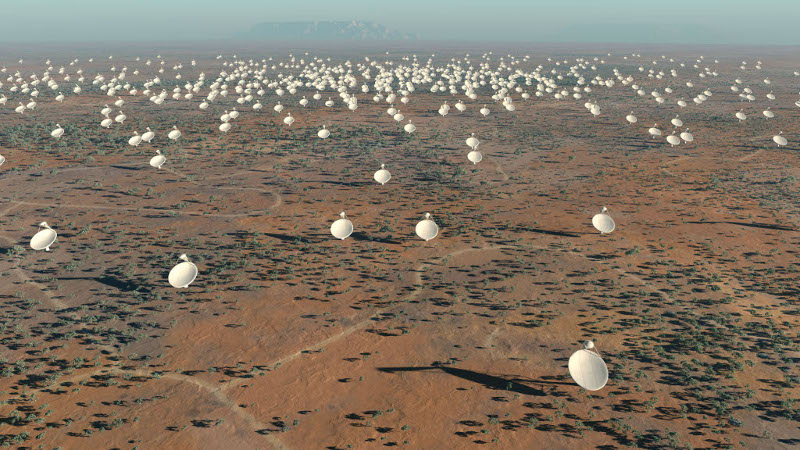
\includegraphics[width=11cm,height=8cm]{images/ska.jpg}\\
\caption{Artist's impression of the SKA dishes. Credit: SKA Organisation/TDP/DRAO/Swinburne Astronomy Productions}
\end{figure}

\subsection{Figures and facts}

The recent launch of the Murchison Widefield Array (MWA) - a radio telescope based in Western Australia's Mid West - marked the start of an impressive flow of astronomical data that will be stored in the iVEC-managed Pawsey Center in Kensington.\\

According to Professor Andreas Wicenec, from The University of Western Australia node of the International Centre for Radio Astronomy Research (ICRAR), SKA has ``now have more than 400 megabytes per second of MWA data streaming along the National Broadband Network from the desert 800 km away''. \footnote{\url{http://www.skatelescope.org/news/pawsey-centre/}} \\

The Murchison Widefield Array is the first Square Kilometre Array precursor to enter full operations, generating a vast torrent of information that needs to be stored for later retrieval by researchers.\\

According to Proffesor Wicenec, ``To store the Big Data the MWA produces, you’d need almost three 1 TB hard drives every two hours`. The technical challenge isn’t just in saving the observations but how you then distribute them to astronomers from the MWA team in far-flung places so they can start using it''.\\

There are currently two links between the data stores in Perth and MWA researchers at the Massachusetts Institute of Technology (MIT) in the United States and the Victoria University of Wellington in New Zealand. A future link to India — another MWA partner — will also be created.\\

The data are not obviously intented to be fully available for everybody at everytime: for instance, MIT researchers are interested in the early universe so filtering techniques to control what data is copied from the Pawsey Center archive to the MIT machines are used. By 2013, more than 150 TB of data had been transferred automatically to the MIT store, with a stream of up to 4 TB a day increasing that value.\\

MWA is producing so much information that it would be impossible to manually decide where to send what, which is where a sophisticated archiving system — the open-source Next Generation Archive System (NGAS) — comes in. NGAS was initially developed by Professor Wicenec at the European Southern Observatory (ESO) and later modified by the ICRAR team to meet the MWA data challenge.\\

In the NGAS one simply asks the system for what the data wanted and it either provides it from the local store or retrieves it from the full archive back in Perth.\\

About half of all MWA computing occurs on site in the Murchison, where signals from radio telescope antennas are combined and processed in a powerful system of computers called a correlator. What's left to do in Perth is produce images, and manage storage and distribution by the archive system so MWA astronomers can analyze the collected data. Data travels down a dedicated 10 gigabit per second connection between the Murchison Radio-astronomy Observatory (MRO) and Geraldton, and the trip to Perth is completed on Australia’s new high-speed National Broadband Network.\\

The MWA will store about 3 Petabytes at the Pawsey Center each year. Another section of the Pawsey Center will be a supercomputing facility that includes computing for Australia's other SKA precursor, CSIRO’s Australian Square Kilometre Array Pathfinder (ASKAP), and projects from geoscience and other computationally intensive fields.\\

To sum up, some relevants figures and facts about SKA:

\begin{itemize}

\item The data collected by the SKA in a single day would take nearly two million years to playback on an ipod.
\item The SKA central computer will have the processing power of about one hundred million PCs.
\item The SKA will use enough optical fibre to wrap twice around the Earth.
\item The dishes of the SKA will produce 10 times the global internet traffic.
\item The SKA will generate enough raw data to fill 15 million 64 GB iPods every day.
\item The SKA will be so sensitive that it will be able to detect an airport radar on a planet 50 light years away.
\item Analysts estimate the London Olympics was the most data-heavy yet - with some 60 Gbytes, the equivalent of 3,000 photographs, travelling across the network in the Olympic Park every second. This however is only equivalent to the data rate from about half a low frequency aperture array station in SKA phase one.

\end{itemize}